%\documentclass[aps,physrev,10pt,floatfix,reprint]{revtex4-2}
\documentclass[10pt, notitlepage]{revtex4-2}

\usepackage{graphicx}% Include figure files
\usepackage{dcolumn}% Align table columns on decimal point
\usepackage{bm}% bold math
\usepackage{hyperref}% add hypertext capabilities
\usepackage[mathlines]{lineno}% Enable numbering of text and display math
%\linenumbers\relax % Commence numbering lines

\usepackage[%Uncomment any one of the following lines to test 
%scale=0.7, marginratio={1:1, 2:3}, ignoreall,% default settings
%text={7in,10in},centering,
%%margin=1.5in,
total={6.5in,8.75in}, top=1.2in, left=0.5in, right=0.5in, includefoot,
%%height=10in,a5paper,hmargin={3cm,0.8in},
]{geometry}
\usepackage[utf8]{inputenc}
\usepackage{amsmath}
\usepackage{amstext}
\usepackage{graphicx}
\usepackage{esint}
\usepackage{geometry}
\usepackage{hyperref}
\usepackage{amsfonts}
\usepackage{nicefrac}

\hypersetup{
    colorlinks=true,
    linkcolor=blue,
    filecolor=magenta,      
    urlcolor=cyan,
    pdftitle={Overleaf Example},
    pdfpagemode=FullScreen,
    }
%\geometry{verbose,lmargin=2cm,rmargin=2cm}

%% TO WRITE: EXACT FREE ENERGY SOLUTION OF THE CW MODEL
% MONTE CARLO SIMULATION SPEC
% 

\begin{document}

\title{Supplementary information of the: "The autoregressive neural network architecture of the Boltzmann distribution of pairwise interacting spins systems"}

\author{Indaco Biazzo}
\maketitle
\tableofcontents

\section{ANRR architecture of the Curie-Weiss model}

The Curie-Weiss model (CW) is a uniform, fully-connected Ising model. The Hamiltonian of the Curie-Weiss model (CW) with $N$ spins is $H\left(\mathbf{x}\right)=-h\sum_{i=1}^{N}x_{i}-\frac{J}{N}\sum_{i<j}x_{i}x_{j}$. Defining $M_{<i}[\mathbf{x}_{<i}]=\sum_{s=1}^{i-1}x_{s}$ and $M_{>i}=\sum_{l=i+1}^{N}x_{l}$, the conditional probability of a spin $i$, see eq.11 in the main text, of the CW model, is:
\begin{equation}
%\begin{multline}
P^{CW}\left(x_{i}=1|\mathbf{x}_{<i}\right) = 
\sigma\bigg( 
 2 \beta h + 2 \beta \frac{J}{N}M_{i<}[\mathbf{x}_{<i}] + %\\
 \log(\rho_i^+[\mathbf{x}_{<i}]) - \log(\rho_i^-[\mathbf{x}_{<i}])
\bigg),
\label{eq:conditional_cw}
\end{equation}
%\end{multline}
where:
\begin{equation}
\rho_i^{\pm}[\mathbf{x}_{<i}] \propto \sum_{\mathbf{x}_{>i}}e^{\beta \left(h\pm\frac{J}{N}+\frac{J}{N}M_{<i}[\mathbf{x}_{<i}]\right)M_{>i}+\frac{\beta J}{2N}M_{>i}^{2}} 
%\sum_{x_{i+1}\dots x_{N}} e^{\beta h_i^{\pm}[\mathbf{x}_{<i}]S_i +\frac{\beta J}{2N}S_{i}^{2}},
\label{eq:rho_cw_0}
\end{equation}
Defining $h_i^{\pm}[\mathbf{x}_{<i}] =h\pm\frac{J}{N}+\frac{J}{N}M_{<i}[\mathbf{x}_{<i}]$, at given $\mathbf{x}_{<i}$, the eq.\ref{eq:rho_cw_0} is equivalent to the partition function of CW model, with $N-i$ spins and external fields $h_i^{\pm}$, as written in the main text. 
The sums over the configurations of the spins $l$ can be carried on easily: 
\begin{multline}
 \rho_i^{\pm}[\mathbf{x}_{<i}] = \sum_{x_{i+1}\dots x_{N}} e^{\beta h_i^{\pm}[\mathbf{x}_{<i}]M_{>i} +\frac{\beta J}{2N}M_{>i}^{2}} = \sqrt{\frac{N}{2\pi \beta J}}\sum_{x_{i+1}\dots x_{N}}e^{\beta h_i^{\pm}[\mathbf{x}_{<i}] M_{>i}}\int e^{-\frac{N}{2J \beta}t^{2}+t M_{>i}} dt\\
  = \sqrt{\frac{N}{2\pi \beta J}}\int dt e^{-\frac{N}{2J \beta}t^{2}} \sum_{x_{i+1}\dots x_{N}}e^{(\beta h_i^{\pm}[\mathbf{x}_{<i}] + t) M_{>i}}  
 =  \sqrt{\frac{N}{2\pi \beta J}}\int dt e^{-\frac{N}{2J \beta}t^{2}} \left(e^{\beta h_i^{\pm}[\mathbf{x}_{<i}] + t} + e^{ (-\beta h_i^{\pm}[\mathbf{x}_{<i}] - t)} \right)^{N-i}  \\ 
 \label{eq:rho_last_exact}
 \end{multline} 
 where we used the Hubbard–Stratonovich (HS) transformation to obtain the second equality. The last equality is obtained just by summing over the variables $x_l$.\\
 First, in the following, we derive the exact feed-forward representation of eq.\ref{eq:conditional_cw} at finite $N$ number of variables, then in the limit of $N\rightarrow \infty$.\\

 \subsection{Exact expression of the conditional probability of the CW model}
 The integral in the equation \ref{eq:rho_last_exact} can be computed the following way:

 \begin{eqnarray*}
 \rho_i^{\pm}[\mathbf{x}_{<i}] &=& \sqrt{\frac{N}{2\pi \beta J}}\int dt e^{-\frac{N}{2J \beta}t^{2}} 
 \sum_{k=0}^{N-i} \binom{N-i}{k} e^{(N-i-2k)*(\beta h_i^{\pm}[\mathbf{x}_{<i}] + t)}\\
 &=& \sum_{k=0}^{N-i} \binom{N-i}{k} \sqrt{\frac{N}{2\pi \beta J}}\int dt e^{-\frac{N}{2J \beta}t^{2}} 
  e^{(N-i-2k)*(\beta h_i^{\pm}[\mathbf{x}_{<i}] + t)}\\
&=& \sum_{k=0}^{N-i} \binom{N-i}{k}e^{\frac{\beta J}{2N}\left(N-i-2k\right)^{2}+\left(N-i-2k\right)\left(\beta h \pm \frac{\beta J}{N}\right)} e^{\frac{\beta J}{N}\left(N-i-2k\right) \sum_s x_s} \\
&=& \sum_{k=0}^{N-i} e^{a_{i,k}^{\pm} + b_{i,k}^{\pm} \sum_s x_s} 
\end{eqnarray*}
where:
\begin{eqnarray}
\label{eq:params}
e^{b_{i,k}^{\pm}} & = & \binom{N-i}{k}e^{\frac{\beta J}{2N}\left(N-i-2k\right)^{2}+\left(N-i-2k\right)\left(\beta h \pm \frac{\beta J}{N}\right)}\\
e^{\omega_{i,k}^{\pm}} & = & e^{\frac{\beta J}{N}\left(N-i-2k\right)},
\end{eqnarray}
proving the equation shown in the main text.

\subsection{Thermodynamical limit of the conditional probability of the CW model}
In the thermodynamical limit, the Curie-Weiss model admits an analytical solution. The order parameter of the system is the magnetization, $m_{\beta}=\frac{1}{N Z}\sum_{\mathbf{x}}\sum_i x_i e^{-\beta H}$ with $Z = \sum_{\mathbf{x}} e^{-\beta H}$. At high temperatures, with zero external fields $h=0$, the magnetization, $m_{\beta}$, is zero up to a critical temperature $\beta_c=\frac{1}{J}$, where a phase transition occurs, and a non-zero magnetization is observed \cite{kadanoff2000statistical}. Considering the following variables: $\eta_i = \frac{N-i}{N}$, $m_i = -\frac{N-i-2k}{N}$, and for simplicity, the $h=0$ case, we can rewrite the expression, eq.\ref{eq:rho_last_exact}, as:
%\begin{widetext}
\begin{align}
    \rho_i^{\pm}[\mathbf{x}_{<i}] &= \sqrt{\frac{N}{2\pi \beta J}}\int dt e^{-\frac{N}{2J \beta}t^{2}} 
    \sum_{k=0}^{N-i} \binom{N-i}{k} e^{(N-i-2k)*(\beta h_i^{\pm}[\mathbf{x}_{<i}] + t)}\\ \label{eq:rho_last_exact2} &= \sum_{k=0}^{N-i} \binom{N-i}{k}e^{\frac{\beta J}{2N}\left(N-i-2k\right)^{2}+\left(N-i-2k\right)\left(\pm\frac{\beta J}{N}\right)} e^{\frac{\beta J}{N}\left(N-i-2k\right) \sum_s x_s}  \\
    &= \sum_{m_i=-\eta_i}^{\eta_i} \binom{N \eta_i}{\frac{N(m_i+\eta_i)}{2}} e^{\frac{N \beta J}{2}m_i^{2} \mp \beta J m_i } e^{N \eta_i \beta J \frac{\sum_s x_s}{N-i}}
\end{align}    
%\end{widetext}

In the limit $N \gg 1$, and using the Stirling approximation for the binomial factor, we obtain:
 \begin{align}
 \rho_i^{\pm} & = 
  \int_{-\eta_i}^{\eta_i} \binom{N\eta_i}{\frac{N(m_i+\eta_i)}{2}} e^{\frac{N \beta J}{2}m_i^{2} \mp \beta J m_i } e^{N \eta_i \beta J \frac{\sum_s x_s}{N-i}} dm_i \\
\begin{split} 
  = & \int_{-\eta_i}^{\eta_i} \exp\bigg\{-N\eta_i \big( -\frac{1+\frac{m_i}{\eta_i}}{2} \log\frac{1+\frac{m_i}{\eta_i}}{2} \\
   & - \frac{1-\frac{m_i}{\eta_i}}{2} \log\frac{1-\frac{m_i}{\eta_i}}{2} 
      - \frac{\beta m_i^2}{2 \eta_i} + \beta m_i \frac{\sum_s x_s}{N-i}\big) \bigg\} e^{\mp \beta J m_i} dm_i
\end{split} \\
\begin{split} 
  \approx & \exp\bigg\{-N\eta_i \big( -\frac{1+\frac{\tilde{m}_{i}}{\eta_i}}{2} \log\frac{1+\frac{\tilde{m}_{i}}{\eta_i}}{2} \\
   & - \frac{1-\frac{\tilde{m}_{i}}{\eta_i}}{2} \log\frac{1-\frac{\tilde{m}_{i}}{\eta_i}}{2} 
      - \frac{\beta \tilde{m}_{i}^2}{2 \eta_i} + \beta \tilde{m}_{i} \frac{\sum_s x_s}{N-i}\big) \bigg\} e^{\mp \beta J \tilde{m}_{i}} \\
    \doteq & e^{\mp \beta J \tilde{m}_{i}} 
\end{split}
\end{align}
Where in the third line I used the saddle point method, assuming $N\gg 1$, where $\tilde{m}_{i}$ is the extreme of the function inside the curly brackets. In the last line, I simplify all the elements that are equal between $\rho_i^{+} $ and $\rho_i^{-}$ that cancel each other in the conditional probability function eq.\ref{eq:conditional_cw}. Deriving by $m_i$ the function inside the curly brackets, we obtain that the extreme $\tilde{m}_{i}$ should satisfy the following equation:
\begin{equation}
\frac{\tilde{m}_{i}}{\eta_i} = \tanh \left( \beta(\frac{\tilde{m}_{i}}{\eta_i} - \frac{\sum_s x_s}{N-i}) \right)
\label{eq:extrem_i}
\end{equation}
In the $N$ large limit, and for a typical sample, I assume that: $\frac{\sum_s x_s}{N-i} \approx |\tilde{m}_{\beta}| \text{sgn}(\sum_s x_s)$, where the $m_{\beta}$ is the magnetization of the Curie-Weiss system at inverse temperature $\beta$ and $\text{sgn(x)} = \frac{|x|}{x}$ is the sign function.
We can distinguish two cases when the magnetization of the system is zero or not. 
In the first case, when $\beta\leq 1/J$, the solution of eq.\ref{eq:extrem_i} is zero as well, and $\log(\rho_i^{+}) - \log(\rho_i^{-})=0$ because the only term that makes the two quantities different, $\mp \beta J m_i$, vanish.\\ 
When instead the system acquires a magnetization $m_{\beta}$ different from zero, the eq.\ref{eq:extrem_i} admit one maximum that depends on the two possible symmetric values of $\frac{\sum_s x_s}{N-i}\approx |\tilde{m}_{\beta}| \text{sign}(\sum_q x_q)$. 
The solution of eq.\ref{eq:extrem_i}, $\pm \tilde{m}_{\text{extrem}}$ depends again on $\text{sign}(\sum_s x_s)$, and we can write the maximum solution as $\tilde{m}_{i}=|\tilde{m}_i| \text{sgn}(\sum_s x_s)$. 
Easily we obtain that $\log(\rho_i^{+}) - \log(\rho_i^{-}) = -2\beta J|\tilde{m}_i| \text{sgn}(\sum_s x_s)$, demostrating the formula in the main text.

\section{Analytic expression of the Curie-Weiss free energy at finite N}
The free energy of a system is defined as:
\begin{equation}
F = -\frac{1}{\beta} \log Z
\end{equation}
For the CW system, with similar computation that leads to the eq.\ref{eq:rho_last_exact2}, we find:
\begin{equation}
F = -\frac{1}{\beta}\log \sum_{k=0}^{N} \binom{N}{k}e^{\frac{\beta J}{2}\left(N-2k\right)^{2}+\left(N-2k\right)h}  + \frac{J}{2}
\end{equation}

\section{ANRR architectures of The Sherrington-Kirkpatrick model}
In order to derive the architecture for the SK model based on the replica method, I'll start from the eq.17 presented in the main text:
\begin{equation}
\mathbb{E}_{\underline{J}}\left[(\rho_i^{\pm}[\mathbf{x}_{<i}])^n \right]  = \\
\int \prod_{l<l'} dP_{J_{ll'}} \bigg\{ 
\sum_{\{\underline{x}^{a}\}_{i+1}^N} \exp\bigg[\beta \bigg(
\sum_{l,a}\bigg( \pm J_{il} + \sum_{s} J_{sl} x_s \bigg) x_l^{a} + 
\sum_{l,l', a} J_{ll'} x_l^{a} x_{l'}^{a}
\bigg)  \bigg] 
\bigg\}
\end{equation}
where, the sums over $(l,l')$, $s$ and $a$ run respectively over $(i+1,N)$, $(1,i-1)$ and $(1,n)$, and $dP_{J_{ll'}}=P(J_{ll'})dJ_{ll'}$. Here we assumed that $N-i \gg 1$, and the average over the disorder $\mathbb{E}_{\underline{J}}$ is on the parameters $J_{l,l'}$ with $l,l'>i$. Defining $h_l^{\pm}[\mathbf{x}_{<i}] =\pm J_{il} + \sum_{s=1}^{i-1} J_{sl} x_s$ as an external field, we can observe that the above quantity is the partition function of the SK model on $\mathbf{x}_{i>}$ variables, with external fields $h_l^{\pm}[\mathbf{x}_{<i}]$, at fixed $\mathbf{x}_{<i}$, and $J_{ll'}$ as coupling constants. \\  
Computing the integrals over the disorder variables $\{J_{ll'}\}$ yields:
\begin{widetext}
\begin{eqnarray}
\mathbb{E}_{\underline{J}}\left[(\rho_i^{\pm}[\mathbf{x}_{<i}])^n \right] & = & 
\sum_{\{\underline{x}^{a}\}_{i+1}^N} 
\exp\left\{\beta \left[
\sum_{l} h_l^{\pm}[\mathbf{x}_{<i}] \sum_{a} x_l^{a} +\frac{\beta}{2N} \sum_{l,l'} \sum_{a,b} x_l^{a} x_l^{b} x_{l'}^{a}x_{l'}^{b} \right]  \right\} \\
& = & e^{ \frac{(N-i) \beta^2}{4N}((N-i)n-n^2) } 
\sum_{\{\underline{x}^{a}\}_{i+1}^N} 
\exp\left\{\beta \left[
\sum_{l} h_l^{\pm}[\mathbf{x}_{<i}] \sum_{a} x_l^{a} +\frac{\beta}{2N} \sum_{a<b} \left( \sum_{l}  x_l^{a} x_l^{b} \right)^2 \right]  \right\}
\end{eqnarray}
\end{widetext}
Using the Hubbard-Stratonovich transformation of the quadratic terms, we can write:
\begin{widetext}
\begin{eqnarray}
\mathbb{E}_{\underline{J}}\left[(\rho_i^{\pm}[\mathbf{x}_{<i}])^n \right] & = & 
c(n,N,i)
\int \prod_{a<b} dQ_{ab} e^{-\frac{N}{2}\beta^2Q_{a,b}^2}
\sum_{\{\underline{x}^{a}\}_{i+1}^N} 
\exp\left\{\beta \left[
\sum_{l} h_l^{\pm}[\mathbf{x}_{<i}] \sum_{a} x_l^{a} +\beta \sum_{a<b} Q_{a,b} \sum_{l}  x_l^{a} x_l^{b} \right]  \right\} \\
& = & 
c(n,N,i)
\int \prod_{a<b} dQ_{ab} e^{-\frac{N}{2}\beta^2Q_{a,b}^2}
\prod_{l} \left[
\sum_{\{\underline{x}^{a}_l\}} 
\exp\left\{\beta \left[
h_l^{\pm}[\mathbf{x}_{<i}] \sum_{a} x_l^{a} +\beta \sum_{a<b} Q_{a,b}  x_l^{a} x_l^{b} \right]  \right\}
\right] \label{eq:before_ansaltz}
\end{eqnarray}
\end{widetext}
where we defined: 
$$c(n,N,i) = e^{ \frac{(N-i) \beta^2}{4N}((N-i)n-n^2) } \left(\frac{2\pi \beta^2}{N}\right)^{\frac{n(n-1)}{2}}.$$ 
The Parisi solutions of the SK model prescribe how to parametrize the matrix of the overlaps $Q$ \cite{10.1142/0271}. The following shows how to obtain neural network architectures based on the replica symmetric (RS) and k-step replica symmetric broken (k-RSB) solutions.

\subsection{Replica Symmetric solution (RS)}
\label{sec:RS}
We assume that the overlaps between the replicas are symmetric under permutations, and the matrix of the overlaps between replicas is parametrized with only one variable $q$:
$$
Q_{a,b}=\begin{cases}
			0, & \text{if $a=b$}\\
            q, & \text{otherwise}
		 \end{cases},
$$
obtaining:
\begin{widetext}
\begin{eqnarray}
\mathbb{E}_{\underline{J}}\left[(\rho_i^{\pm, sym}[\mathbf{x}_{<i}])^n \right] & = & 
c(n,N,i)
\int dq e^{-\frac{n(n-1)N}{4}\beta^2 q^2}
\prod_{l} \left[
\sum_{\{\underline{x}^{a}_l\}} 
\exp\left\{\beta \left[
h_l^{\pm}[\mathbf{x}_{<i}] \sum_{a} x_l^{a} +\beta q \sum_{a<b} x_l^{a} x_l^{b} \right]  \right\} 
\right] \\
& = &
c(n,N,i)
\int dq e^{-\frac{n(n-1)N}{4}\beta^2 q^2}
e^{-\frac{nN\beta^2 q}{2}}
\prod_{l} \left[
\sum_{\{\underline{x}^{a}_l\}} 
e^{\beta \left[
h_l^{\pm}[\mathbf{x}_{<i}] \sum_{a} x_l^{a} + \frac{\beta q}{2} \left(\sum_{a} x_l^{a} \right)^2 \right]} 
\right]\\
& = &
c'(n,N,i)
\int dq e^{-\frac{n(n-1)N}{4}\beta^2 q^2}
e^{-\frac{nN\beta^2 q}{2}}
\prod_{l} \left[\int \frac{dz_l}{\sqrt{2\pi q}} e^{-\frac{z_l^2}{q}}
\sum_{\{\underline{x}^{a}_l\}} 
e^{\beta \left(
h_l^{\pm}[\mathbf{x}_{<i}] +\beta z_l \right) \sum_{a} x_l^{a}} 
\right]\\
& = &
c'(n,N,i)
\int dq e^{-nN\left(\frac{(n-1)}{4}\beta^2 q^2 +\frac{\beta^2 q}{2}\right)}
\prod_{l} \left[\int \frac{dz_l}{\sqrt{2\pi q}} e^{-\frac{z_l^2}{q}}
2^n\cosh^n \left(\beta \left(
h_l^{\pm}[\mathbf{x}_{<i}] +\beta z_l \right)\right) 
\right].\\
\end{eqnarray}
\end{widetext}
Using the limit that $n\rightarrow 0$ we can write:
\begin{widetext}
\begin{eqnarray}
\int \frac{dz_l}{\sqrt{2\pi q}} e^{-\frac{z_l^2}{q}}
2^n\cosh^n \left(\beta \left(
h_l^{\pm}[\mathbf{x}_{<i}] +\beta z_l \right)\right) = e^{n \int \frac{dz_l}{\sqrt{2\pi q}} e^{-\frac{z_l^2}{q}}
\log 2\cosh \left(\beta \left(
h_l^{\pm}[\mathbf{x}_{<i}] +\beta z_l \right)\right)}.
\label{eq:gauss_n0}
\end{eqnarray}
\end{widetext}
obtaining:
\begin{widetext}
\begin{eqnarray}
\log (\rho_i^{\pm, sym}[\mathbf{x}_{<i}]) & = & 
\lim_{n\rightarrow 0} \frac{1}{n} \log \left( c'(n,N,i)
\int dq e^{-\frac{n(n-1)N}{4}\beta^2 q^2}
e^{-\frac{nN\beta^2 q}{2}}
e^{n \sum_l 
\int \frac{dz_l}{\sqrt{2\pi q}} e^{-\frac{z_l^2}{q}}
\log 2\cosh \left(\beta \left(
h_l^{\pm}[\mathbf{x}_{<i}] +\beta z_l \right)\right)
} 
\right)\\
& = &
\log(c''(N,i)) + 
\left( +\frac{N}{4}\beta^2 q^2_0 
-\frac{N\beta^2 q_0}{2}
+ \sum_l 
\int \frac{dz_l}{\sqrt{2\pi q_0}} e^{-\frac{z_l^2}{q_0}}
\log 2\cosh \left(\beta \left(
h_l^{\pm}[\mathbf{x}_{<i}] +\beta z_l \right)\right)
\right) \\
& \doteq &  
c(N,i, q_0) -
\sum_l 
\int \frac{dz_l}{\sqrt{2\pi q_0}} e^{-\frac{z_l^2}{q_0}}
\log \sigma \left(\beta \left(
2h_l^{\pm}[\mathbf{x}_{<i}] +2\beta z_l \right)\right)
\end{eqnarray}
\end{widetext}
In the second line, I use the saddle point methods to evaluate the integral over $q$, assuming that the single maximum value $q_0$ does not depend on the input values $\mathbf{x}_{<i}$ in the set of $h_l^{\pm}[\mathbf{x}_{<i}]$. It is a bold assumption to be verified {\it a posteriori} on the quality of the neural network architectures performances. 
In the third line, we use the identity $\log\cosh(x) = 2x - \log\sigma(2x)$ and the elements that are equals between $\log(\rho^+)$ and $\log(\rho^-)$ are simplified. We introduced the $\log\sigma$ non-linear operator for computational reasons.

% We can, after some manipulations, obtain a more neural network friendly function:
% \begin{eqnarray}
% \log (\rho_i^{\pm, sym} [\underline{x_l}])^n] & \approx & 
% \text{Extr}_q \left( +\frac{N}{4}\beta^2 q^2 
% -\frac{N\beta^2 q}{2}
% + \sum_l 
% \int dz_l e^{-z_l^2}
% \log \cosh \left(\beta \left(
% h_l +\beta \sqrt{q}z_l \right)\right)
% \right) 
% \end{eqnarray}

Now we consider the following approximation of the Gaussian convolution:
\[
\int dz e^{-z^2}
\log \sigma \left(\beta \left(
h +\beta \sqrt{q}z \right)\right) \sim b_0 + w_0*\log \sigma(b_1 + w_1 h), 
\]
where $(b_0, w_0, b_1,w_1)$ are free parameters to be determined. In the sec.\ref{sec:num_evidence} of the SI a numerical analysis of the quality of this approximation is shown. 
Putting together all the pieces, we can parameterize the conditional probability as:
\begin{multline}
Q^{RS}\left(x_{i}=1|\mathbf{x}_{<i}\right) = \sigma\left( 
    x_i^1(\mathbf{x}_{<i}) +\log(\rho_i^+) - \log(\rho_i^-)
\right) \\
 = \sigma \bigg( x_i^1(\mathbf{x}_{<i}) + \sum_{l^+=i+1}^{N}  w_0^{i,l^+} \log\sigma(b_1^{i,l^+} +
 w_1^{i,l^+} x_{i,l^+}^1(\mathbf{x}_{<i}))+ 
 + \sum_{l^-=i+1}^{N}  w_0^{i,l^-} \log\sigma(b_1^{i,l^-} + w_1^{i,l^-} x_{i,l^-}^1(\mathbf{x}_{<i})
 \bigg) 
\end{multline}
where the set of $(\mathbf{b},\mathbf{w})$ are free variational parameters to learn in the training process. 
%The $\sum_l$ considers all the elements together of the plus and minus $\rho^{\pm}$ function. 

\subsection{K-step Replica symmetric breaking (k-RSB)}
\label{sec:rsb}
Assuming that the replica symmetry is broken, we can use the  ansatz called 1-step replica symmetric breaking (1RSB), where the overlaps between replicas are divided into $m$ blocks:
\begin{eqnarray}
    Q_{a,b}=\begin{cases}
			q_1, & \text{if } I(a/m)=I(b/m) \\
            q_0. & \text{if } I(a/m) \neq I(b/m).
		 \end{cases}
\end{eqnarray}
With the above ansatz, we can compute the following quantities:
\begin{align}
\begin{split}
    \sum_{ab} Q_{ab} x_{a} x_{b}  &  = \frac{1}{2} \bigg[ q_0 \left( \sum_{a}x_a\right)^2 +  (q_1-q_0) \sum_{\text{blocks}}  \left( \sum_{a \in \text{block}}x_a\right)^2   - nq_1\bigg] 
\end{split}
\\
\sum_{ab} Q_{ab}^2 & =  n^2 q_0^2 + nm(q_1^2 - q_0^2) -n q_1^2.
\end{align}
The equation \ref{eq:before_ansaltz} becomes:
%\begin{widetext}
\begin{align*}
& \mathbb{E}_{\underline{J}} \left[(\rho_i^{\pm, 1RSB})^n \right] =  \\[1ex]
\begin{split}
& = c(n,N,i) \int dq_1 dq_0 e^{\frac{N}{2}\beta^2 \left[n^2 q_0^2 + nm(q_1^2 - q_0^2) -n q_1^2 \right]} 
\prod_{l} \bigg[ \sum_{\{\underline{x}^{a}_l\}} e^{ \beta \big[ h_l^{\pm} \sum_{a} x_l^{a} +\beta q_0 \left( \sum_{a} x_p^{a} \right)^2 + \beta (q_1-q_0) \sum_{\text{blocks}} \left( \sum_{a \in \text{block}}x_l^{a}\right)^2  -n q_1 \bigl]}  \bigg] 
\end{split}\\ 
\begin{split}
& = c(n,N,i) \int dq_1 dq_0 e^{\frac{N}{2}\beta ^ 2 \left[n^2 q_0^2 + nm(q_1^2 - q_0^2) -n q_1^2 -n q_1\right]} 
\prod_{l} \bigg[ \sum_{\{\underline{x}^{a}_l\}} \int dP_{z_l} \prod_{k=1}^{n/m} \int dP{y_{lk}}  e^{\beta \big[h_l^{\pm} \sum_{a} x_l^{a} + \beta z_l \sum_{a}x_l^{a} + \beta \sum_{\text{blocks}}  y_{lk} \sum_{a \in \text{block}}x_l^{a}\bigl]}  \bigg] 
\end{split}\\ 
\begin{split}
& = c(n,N,i) \int dq_1 dq_0 e^{\frac{N}{2}\beta^2 \left[n^2 q_0^2 + nm(q_1^2 - q_0^2) -n q_1^2 -n q_1\right]} 
\prod_{l} \bigg[ \int dP_{z_l}  \prod_{k=1}^{n/m} \int dP_{y_{lk}} \cosh^m\bigg(\beta \big[h_l^{\pm}+ \beta z_l +\beta y_{lk}\bigl]  \bigg)  \bigg]
\end{split}\\ 
\begin{split}
& = c'(n,N,i) + c(n,N,i) \int dq_1 dq_0 e^{\frac{N}{2}\beta\left[n^2 q_0^2 + nm(q_1^2 - q_0^2) -n q_1^2 -n q_1\right]} 
\prod_{p} \int dP_{z_l}  \exp \bigg\{ \frac{n}{m} \log \bigg( \int dP_{y_{l}} \cosh^m\bigg(\beta \big[h_l^{\pm}+ \beta z_l + \beta y_{l}\bigl]  \bigg)  \bigg) \bigg\},
\end{split}\\ 
\end{align*}
%\end{widetext}
where we defined:
\begin{align}
    dP_{z_l} & = \frac{dz_l}{\sqrt{2\pi q_0}}e^{\frac{z^2}{2q_0}}\\
    dP_{y_{l}} & = \frac{dy_{l}}{\sqrt{2\pi (q_1-q_0)}}e^{\frac{y_{l}^2}{2 (q_1-q_0)}}.
\end{align}
Considering $N \gg 1$ and $n\rightarrow 0$ to use the saddle point methods and the identity in eq.\ref{eq:gauss_n0}, we can write:
\begin{widetext}
\begin{align}
\log (\rho_i^{\pm, 1RSB}) & = 
\lim_{n\rightarrow 0} \frac{1}{n} \log \left(\mathbb{E}_{\underline{J}} \left[(\rho_i^{\pm, 1RSB})^n \right]  \right) \\
& = c_i +  \text{Extr}_{q_0, q_1} \bigg[ c'_i(N,n,q_0, q_1) 
+ \frac{1}{m} \sum_{l} \int dP_{z_l} \log \bigg( \int dP_{y_{l}} \cosh^m\bigg(\beta \big[h_l^{\pm}+ \beta z_l + \beta y_{l}\big]  \bigg)  \bigg)
\bigg].
\end{align}
\end{widetext}

The above integrals are rewritten as the following:
\begin{align}
& \int dP_{z_l} \log \bigg( \int dP_{y_{l}}  \cosh^m\bigg(\beta \big[h_l^{\pm}+\beta z_l + \beta  y_{l}\big]  \bigg)  \bigg) 
 = \\
& \int dP_{z_l} \log \biggl( \int dP_{y_{l}} e^{ m \log \cosh \left(\beta \left[h_l^{\pm}+ \beta  z_l + \beta  y_{l}\right]  \right) } \biggr) 
 = \\
& \beta h_{l}^{\pm} + \int dP_{z_l} \log \biggl( \int dP_{y_{l}} e^{\beta^2 m y_{l} - m \log \sigma \left(\beta \left[h_l^{\pm}+ \beta z_l +\beta y_{l}\right]  \right) } \biggr) 
\end{align}
We have two nested gaussian convolutions.
% In order to make it easier to compute this non-linear operator, we will use a sequence of approximations similar to those used previously for RS case. %Recalling $h_l^{\pm}[\mathbf{x}_{<i}] =\pm J_{il} + \sum_{s} J_{sl} x_s$, we consider the approximation of the nested gaussian convolution:
%\begin{multline}
%f(\mathbf{x}_{<i}) = \int \frac{dz_l}{\sqrt{2\pi q_0}}e^{\frac{z^2}{2q_0}} \log \bigg( \int \frac{dy_{l}}{\sqrt{2\pi (q_1-q_0)}}e^{\frac{y_{l}^2}{2 (q_i-q_0)}} \\
% e^{ y_{l} - m \log \sigma \left(\beta \left[\pm J_{il} + \sum_{s} J_{sl} x_s + h + z_l + y_{l}\right]  \right) } \bigg) 
%\end{multline}
%Fixed the parameters of the model $(\{J_{pq}\}, h, \beta)$, this is a function that depends from three free parameters $(q_0, q_1, m)$. 
The integrals over the variables $(z_l, y_l)$ are approximated in the same way as the approach used previously for RS case: the number of free parameters increases to have feed-forward functions without integrals. First, we consider the following maps:
\begin{align}
    & \log \int dP_{y_{l}} e^{ \beta^2 m y_{l} - m \log \sigma \left(\beta \left[h_l^{\pm}+\beta z_l +\beta y_{l}\right]  \right) }  \approx\\
    & \log \bigg( \hat{b}_0^{l^{\pm}} + \hat{w}_0^{l^{\pm}} e^{\hat{b}_1^{l^{\pm}} + \hat{w}_1^{l^{\pm}} \log \sigma (\hat{b}_2^{l^{\pm}} + \hat{w}_2^{l^{\pm}} (h_l^{\pm}+ \beta  z_l))} \bigg) = \\
    & \log(b_0^{l^{\pm}}) + \log(1 + e^{ \log( \frac{\hat{w}_0^{l^{\pm}}}{b_0^{l^{\pm}}} ) + \hat{b}_1^{l^{\pm}} + \hat{w}_1^{l^{\pm}} \log \sigma (\hat{b}_2^{l^{\pm}} + \hat{w}_2^{l^{\pm}} (h_l^{\pm}+ \beta  z_l))})=\\
    & \log(\hat{b}_0^{l^{\pm}}) - \log\sigma( \log( \frac{\hat{w}_0^{l^{\pm}}}{b_0^{l^{\pm}}} ) + \hat{b}_1^{l^{\pm}} + \hat{w}_1^{l^{\pm}} \log \sigma (\hat{b}_2^{l^{\pm}} + \hat{w}_2^{l^{\pm}} (h_l^{\pm}+ \beta  z_l)))=\\
    & b_0^{l^{\pm}} + w_0^{l^{\pm}} \log\sigma(b_1^{l^{\pm}} + w_1^{l^{\pm}} \log \sigma (b_2^{l^{\pm}} + w_2^{l^{\pm}} (h_l^{\pm}+ \beta  z_l)))
%        \int dx e^{\frac{x^2}{a}} \log\sigma (a_1 + b_1 \log \sigma (a_2 + b_2 (h+x))) & \approx a_0 +b_0 \log \sigma (a'_1 + b'_1 \log \sigma (a'_2 + b'_2 (h))) 
\end{align}
Where in the last equation I renamed the variational parameters, for instance, $ b_0^{l^{\pm}} = \log(\hat{b}_0^{l^{\pm}})$, $w_0^{l^{\pm}} =-1$, etc. Then once again:
\begin{align}
        & \hat{b}_0^{l^{\pm}} + \hat{w}_0^{l^{\pm}} \int dP_{z_l} \log \sigma \bigg(\hat{b}_1^{l^{\pm}} + \hat{w}_1^{l^{\pm}} \log \sigma (\hat{b}_2^{l^{\pm}} + \hat{w}_2^{l^{\pm}} (h_l^{\pm}+ \beta  z_l)) \bigg) \approx \\
        & b_0^{l^{\pm}} + w_0^{l^{\pm}} \log \sigma (b_1^{l^{\pm}} + w_1^{l^{\pm}} \log \sigma (b_2^{l^{\pm}} + w_2^{l^{\pm}} (h_l^{\pm}))).
%        \int dx e^{\frac{x^2}{a}} \log\sigma (a_1 + b_1 \log \sigma (a_2 + b_2 (h+x))) & \approx a_0 +b_0 \log \sigma (a'_1 + b'_1 \log \sigma (a'_2 + b'_2 (h))) 
\end{align}
The set of parameters $(\mathbf{b_0^{{\pm}}},\mathbf{w_0^{{\pm}}},\mathbf{b_1^{{\pm}}},\mathbf{w_1^{{\pm}}},\mathbf{b_2^{{\pm}}},\mathbf{w_2^{{\pm}}})$ are free parameters to be determined by the learning procedures. The gaussian convolution integrals are substituted by feed-forward non-linear operations, enlarging the space of parameters. In section \ref{sec:num_evidence} numerical evidence for the goodness of the above approximations is shown. For the 1RSB case, we use the following architecture:
\begin{multline*}
    Q^{1RSB}\left(x_{i}=1|\mathbf{x}_{<i}\right) = \sigma\left( 
        x_i^1(\mathbf{x}_{<i}) +\log(\rho_i^+) - \log(\rho_i^-)
    \right) 
     = \sigma \bigg( x_i^1(\mathbf{x}_{<i}) + \\ \sum_{l^+=i+1}^{N}  w_0^{i,l^+} \log\sigma(b_1^{i,l^+} + 
     w_1^{i,l^+} \log\sigma(b_2^{i,l^+} +
     w_2^{i,l^+}  x_{i,l^+}^1(\mathbf{x}_{<i})))+ \sum_{l^-=i+1}^{N}  w_0^{i,l^-} \log\sigma(b_1^{i,l^-} + w_1^{i,l^-} \log\sigma(b_2^{i,l^+} +
     w_2^{i,l^+} x_{i,l^-}^1(\mathbf{x}_{<i})))
     \bigg) 
\end{multline*}   
The generalization of the $\rho^{\pm}$ parametrization to the k-RSB case is straightforward. For instance, for 2-RSB we have:
\begin{equation*}
    \log \rho^{\pm, 2RSB} \left(x_{i}=1|\mathbf{x}_{<i}\right)  =  
   \sum_{l^{\pm}} w_0^{i,l^{\pm}} \log\sigma(b_1^{i,l^{\pm}} +
   w_1^{i,l^{\pm}} \log\sigma(b_2^{i,l^{\pm}} +
    w_2^{i,l^{\pm}}( \log\sigma(b_3^{i,l^{\pm}} +
    w_3^{i,l^{\pm}}x_{i,l^{\pm}}^1(\mathbf{x}_{<i})))))
\end{equation*}


\subsection{Numerical evidence of Gaussian convolution approximations}
\label{sec:num_evidence}
In this section, I show the numerical evidence of some of the approximations used to represent the non-linear operations derived for the SK model. In the RS case, see subsec.\ref{sec:RS}, the non-linear operation is approximated as in the following:
\begin{equation}
    \label{eq:rs_approx}
    f(x) = \int \frac{dz}{\sqrt{2 \pi q_0}} e^{-\frac{z^2}{q_0}}
\log \sigma \left(\beta \left(
x +\beta \sqrt{q}z \right)\right) \sim b_0 + w_0*\log \sigma(b_1 + w_1 h). 
\end{equation}
The results in fig.\ref{fig:rs_approx} of the fit, using the non-linear least squares method, of the $f(x)$ with the l.h.s of the above expression, with free parameters $b_0, w_0, b_1, w_1$, are shown. Fits for different values of $\beta$ and $q_0$, showing the robustness of the approximation used.  In the 1RSB case, see subsection \ref{sec:rsb}, one of the non-linear operations is approximated as in the following:
\begin{equation}
    f(x) = \log \int  \frac{dz}{\sqrt{2 \pi (q_1-q_0)}} e^{-\frac{z^2}{(q_1-q_0)}} e^{ \beta^2 m z - m \log \sigma \left(\beta x+\beta^2 z \right) }  \approx b_0  + w_0  \log\sigma(b_1  + w_1  \log \sigma (b_2  + w_2  x))
    \label{eq:1rsb_approx}
\end{equation}
As before, the function $f(x)$ is fitted with the l.h.s of the above expression, and the results in fig.\ref{fig:1rsb_approx} show the robustness of the approximation used for different values of $(q_1-q_0)$, $m$, and $\beta$.
\begin{figure}[h]
    \centering
    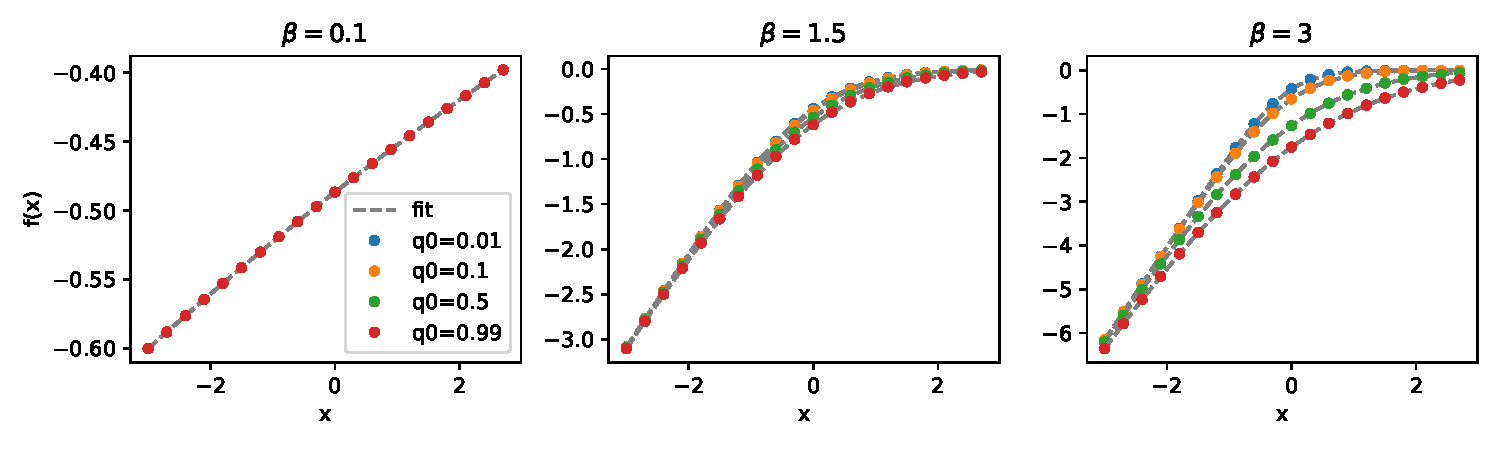
\includegraphics[width=1\textwidth]{img/fit_rs.pdf}
    \caption{Fit of eq.\ref{eq:rs_approx} at different values of $\beta$ and $q_0$. The free parameters are $b_0, w_0, b_1, w_1$. The results show the robustness of the approximation used. }
    \label{fig:rs_approx}
\end{figure}
\begin{figure}[h]
    \centering
    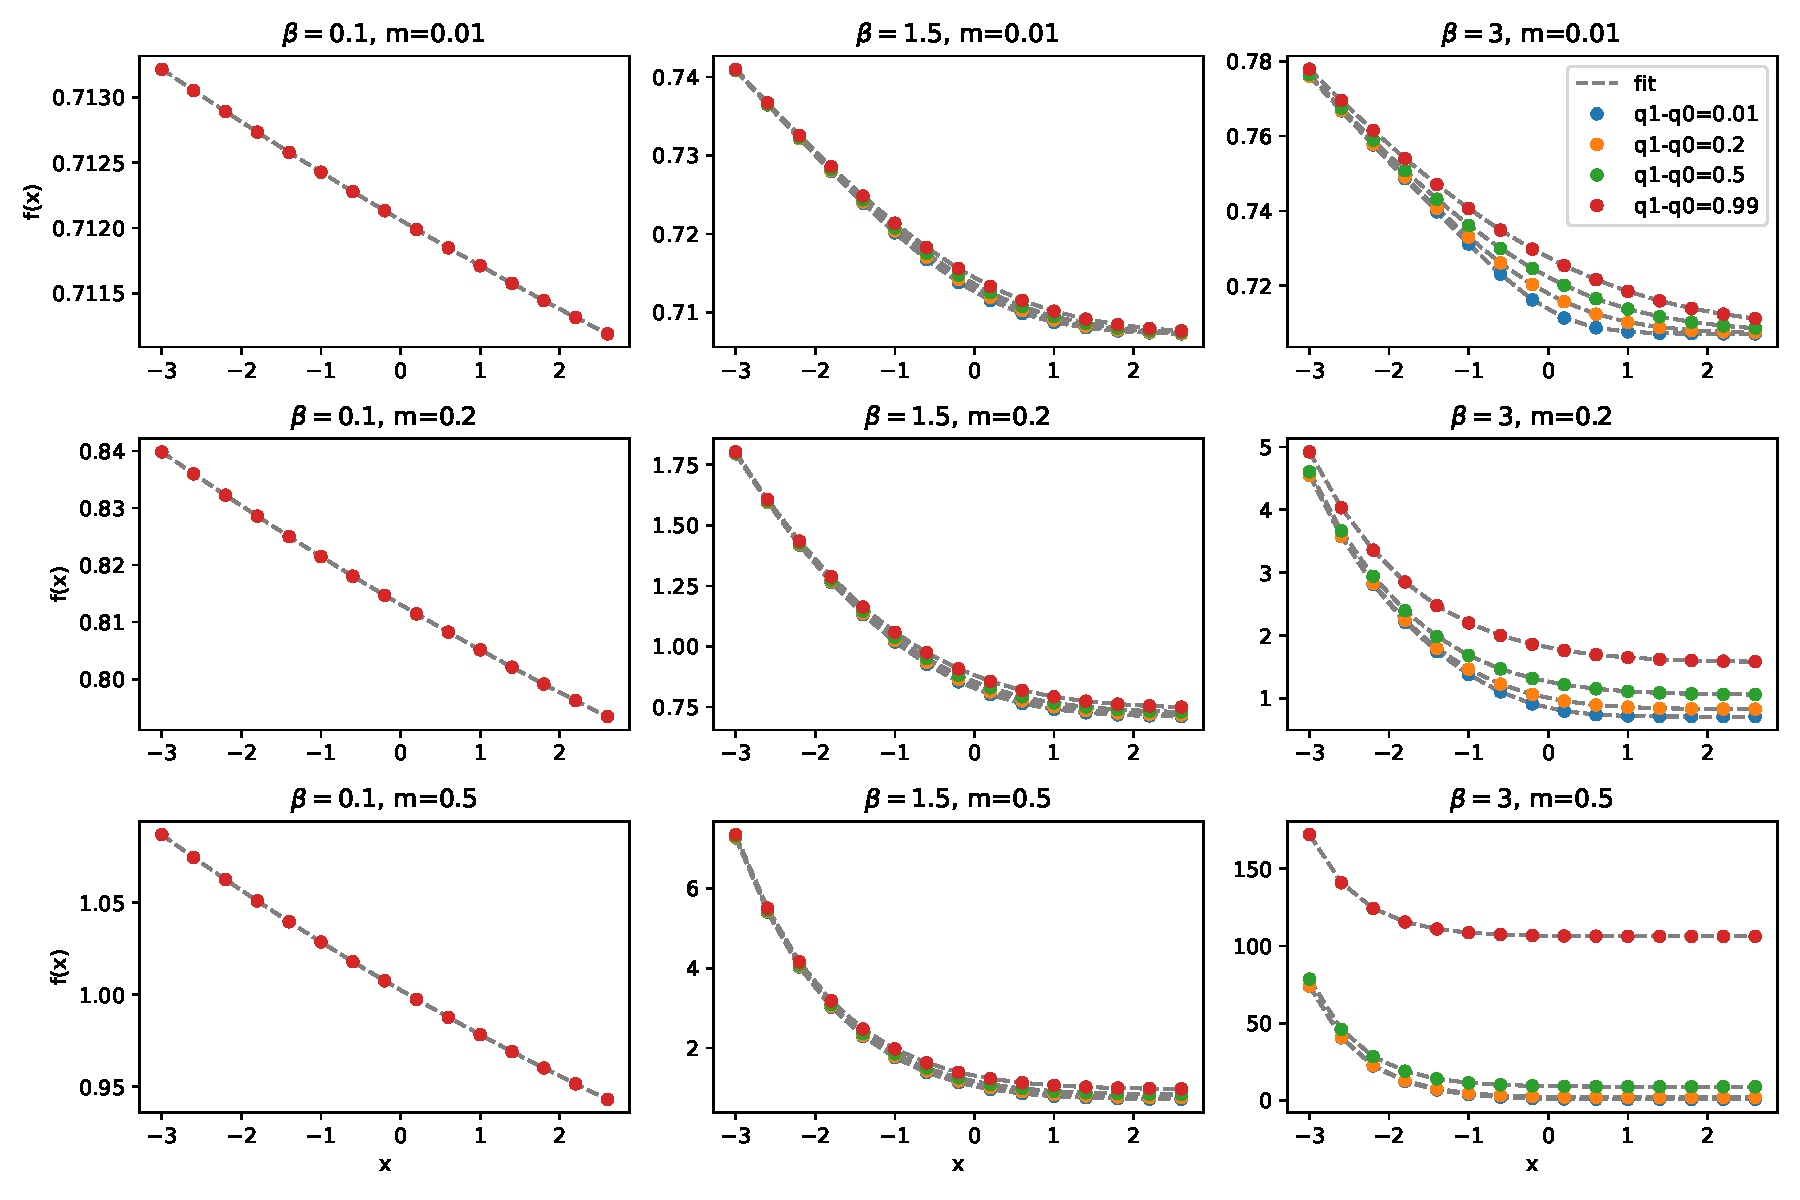
\includegraphics[width=1\textwidth]{img/fit_1rsb.pdf}
    \caption{Fit of eq.\ref{eq:1rsb_approx} at different values of $beta$ $m$, and $q_1 - q_0$. The free parameters are $b_0, w_0, b_1, w_1, b_2, w_2$. The results show the robustness of the approximation used. }
    \label{fig:1rsb_approx}
\end{figure}


\section{Monte Carlo sampling of the SK model}
In the main text, in the section results, in order to check the correlation between the weights of the first layer of the SK$_{1RSB}$ architecture with the coupling of the hamiltonian, 10,000 samples were generated through the Monte-Carlo Metropolis algorithm \cite{doi:10.1063/1.1887186}. The samples are generated for a system with $N=200$ variables at $\beta=2$. Each configuration is sampled after $stf = 200*N$ spin trail flip.  I observe that, for the system under study, for this number of trail spin flips of the Metropolis algorithm the autocorrelation time between the configurations drops below 0.5. The training of the SK$_{1RSB}$ was done minimizing, over the parameters of the SK$_{1RSB}$, the average of the negative log-likelihood (LL) of the generated $m$ samples:
\begin{equation}
    LL = - \frac{1}{m} \sum_{m}\log(Q_{1RSB})
\end{equation}  
\bibliography{main}% Produces the bibliography via BibTeX.

\end{document}
